\documentclass{../../commons/assignment}

\usepackage{float}
\usepackage{tikz}
\usepackage{adjustbox}
\usepackage{titlesec}
\usepackage{soul}
\usepackage{csvsimple}

\usepackage{graphicx}
\usepackage{subcaption}

\usetikzlibrary{calc,patterns,angles,quotes}
\setlength{\parindent}{0pt}

\hypersetup{
pdftitle={ME621 - Advanced Finite Element Methods},
pdfsubject={Report for assignment 1},
pdfauthor={Tommaso Bocchietti}
}

\begin{document}
\graphicspath{{./img/}}


\title{ME621 - Advanced Finite Element Methods \\ Assignment 1}
\author{Tommaso Bocchietti}
\date{A.Y. 2023/24 - W24}

\maketitle

\begin{figure}[H]
    \centering
    
\includegraphics[width=.9\textwidth]{./pdf/UniversityOfWaterloo_logo_vert_pms}
    \label{fig:University_Of_Waterloo_logo}
\end{figure}

\clearpage
\tableofcontents
\listoffigures
\listoftables
\clearpage

\section{Requests}
\label{sec:requests}

A system of two aluminum bars of the same material is shown in the following figure.
The system is subjected to two external loads, $P_x$ and $P_y$, at joint B.
A and C are connected to pinned supports.

\begin{figure}[h]
    \centering
    \begin{tikzpicture}[scale=3]

        \coordinate (A) at (0,0.5);
        \coordinate (B) at (3,0.5);
        \coordinate (Bf) at (3.7,1);
        \coordinate (C) at (3,0);

        % Joint names
        \node at (A) [above, left] {A};
        \node at (B) [below, above] {B};
        \node at (C) [below, left] {C};

        % Initial position
        \draw (A) -- (B) node[midway, below] {$L_1$};
        \draw (C) -- (B) node[midway, left] {$L_2$};

        % Deformed position
        \draw[dashed] (A) -- (Bf)node[midway, above] {$l_1$};
        \draw[dashed] (C) -- (Bf)node[midway, right] {$l_2$};

        % Labels
        \pic [draw, ->, "$\alpha$", angle radius=2cm] {angle = B--A--Bf};
        \pic [draw, <-, "$\beta$", angle radius=0.7cm] {angle = Bf--C--B};

        % Support at the end of Beam 1
        \draw[fill] (0,0.5) circle (0.03);

        % Support at the end of Beam 2
        \draw[fill] (3,0) circle (0.03);

        % Arrows at coordinate Bf
        \draw[->] (Bf) -- ++(0.3, 0) node[right] {$\vec{P_x}$};
        \draw[->] (Bf) -- ++(0, 0.3) node[above] {$\vec{P_y}$};
        \draw[->] (B) -- (Bf) node[midway, above] {$\vec{u}$};
        % \draw[->, shorten >=150pt] (Bf) -- (A) node[above, above] {$\vec{F_1}$};
        % \draw[->, shorten >=50pt] (Bf) -- (C) node[above, right] {$\vec{F_2}$};

    \end{tikzpicture}
    \caption{Problem representation}
    \label{fig:problem_representation}
\end{figure}

The problem asks to:

\begin{itemize}
    \item Obtain the external loads $P_x$ and $P_y$ as a function of horizontal and vertical displacements at point B (namely $u$ and $v$).
    \item Determine the displacements in both $x$ and $y$ directions for $1000$ load increments of $+5\text{N}$ for both $P_x$ and $P_y$ (from zero).
    \item Find the displacement of point B after the final increment.
\end{itemize}

Write a \texttt{MATLAB} code with a convergence error of $10^-5$ to numerically solve the problem.
Use a combination of (a) Euler and N-R, and (b) Euler and modified N-R.
Also plot the resultant force versus the resultant displacement.

Use the Green strain measure:

\begin{equation}
    E_i = \frac{l_i^2 - L^2}{2L^2}
    \label{eq:green_strain_measure_formula}
\end{equation}

From now on, we will refer to the Green strain measure as $\epsilon_{1,2}$ to differentiate it from the Young's modulus $E_{1,2}$.

\begin{table}[H]
    \centering
    \begin{tabular}{|c|c|c|}
        \hline
        \textbf{Parameter} & \textbf{Value} & \textbf{Unit} \\ \hline
        $E_1 = E_2 = E$    & $70$           & $\text{GPa}$  \\ \hline
        $L_1$              & $3$            & $\text{m}$    \\ \hline
        $L_2$              & $0.5$          & $\text{m}$    \\ \hline
        $A_1 = A_2 = A$    & $0.0001$       & $\text{m}^2$  \\ \hline
    \end{tabular}
    \caption{Parameters of the system}
    \label{tab:parameters_of_the_system}
\end{table}

\section{Methodology}
\label{sec:methodology}

We will start by writing the analytical expression of the \textbf{shape functions} for the 4-node element with total length $h_e$ and $\alpha = \beta = \frac{1}{3}$ in terms of the parent coordinate system, $-1 \leq \xi \leq 1$.
To do so, we will make use of \texttt{Mathematica} to perform the symbolic computation and obtain the exact expression of the shape functions.

We will proceed by writing the elemental matrices ($B_0^e$, $f_{int}^e$, $f_{ext}^e$, $f_{kin}^e$) still in terms of the parent coordinate system.

We will then write the \textbf{MATLAB} code to solve the problem implementing the explicit integration scheme with Total Lagrangian finite element formulation and finally plot the deformation of the right end of the bar vs time, namely $u_{end}(t)$.
\section{Solution}

\subsection{Equilibrium equations}

We can start writing the equilibrium equations for the system.
Since we have no data about the mass of the bars, we will assume negligible mass of the bars.
This assumption will allow us to neglect the effect of gravity on the system and avoid the introduction of the inertia terms in the equilibrium equations.

\begin{equation}
    % TODO: check equilibrium equations
    \vec{F_{ext}} + \vec{F_{int}} = \vec{0}
    \label{eq:equilibrium_equations_1}
\end{equation}

\begin{equation}
    \begin{cases}
        \vec{F_{ext}} = \vec{P_x} + \vec{P_y} \\
        \vec{F_{int}} = \vec{F_{int,x}} + \vec{F_{int,y}}
    \end{cases}
\end{equation}

By decomposing the equations in the $x$ and $y$ directions, we obtain:

\begin{equation}
    \begin{cases}
        P_x = F_{int,x} = |F_1|*\cos(\alpha) + |F_2|*\sin(\beta) \\
        P_y = F_{int,y} = |F_1|*\sin(\alpha) + |F_2|*\cos(\beta)
    \end{cases}
    \label{eq:equilibrium_equations_2}
\end{equation}
\subsection{Force displacement relationship}

So far we have obtained the equilibrium equations for the system.
We can now proceed to obtain the force displacement relationship, which will allow us to solve the system of equations ${\vec{P}} = f({\vec{u}})$.
To do so, we try to express everything on the right-hand side of the equilibrium equations in terms of the displacements $u$ and $v$.

From simple trigonometrical considerations, we can obtain the following relationships:

\begin{align}
    \cos(\alpha) & = \frac{\text{L}_1+u}{l_1} \\
    \sin(\alpha) & = \frac{v}{l_1}            \\
    \cos(\beta)  & = \frac{\text{L}_2+u}{l_2} \\
    \sin(\beta)  & = \frac{v}{l_2}
\end{align}

We can now proceed working on the forces, knowing that the internal forces are linked to the strains by the following relationship:

\begin{equation}
    \begin{Bmatrix}
        \vec{F_{int,x}} \\
        \vec{F_{int,y}}
    \end{Bmatrix}
    =
    \begin{Bmatrix}
        \text{A}_1 * \text{E}_1 * \epsilon_1 \\
        \text{A}_2 * \text{E}_2 * \epsilon_2
    \end{Bmatrix}
\end{equation}

And the strains are linked to the displacements by the following relationship:

\begin{equation}
    \begin{Bmatrix}
        \epsilon_1 \\
        \epsilon_2
    \end{Bmatrix}
    =
    \begin{Bmatrix}
        \frac{l_1^2-\text{L}_1^2}{2 \text{L}_1^2} \\
        \frac{l_2^2-\text{L}_2^2}{2 \text{L}_2^2}
    \end{Bmatrix}
\end{equation}

Finally, we can give the following definition to the real length of the bars:

\begin{equation}
    \begin{Bmatrix}
        l_1 \\
        l_2
    \end{Bmatrix}
    =
    \begin{Bmatrix}
        \sqrt{(\text{L}_1+u)^2+v^2} \\
        \sqrt{u^2+(\text{L}_2+v)^2}
    \end{Bmatrix}
\end{equation}

We can now substitute the equations above in the equilibrium equations \ref{eq:equilibrium_equations_2} to obtain the force displacement relationship:

\begin{equation}
    \begin{Bmatrix}
        \vec{P_x} \\
        \vec{P_y}
    \end{Bmatrix}
    =
    \begin{Bmatrix}
        \frac{\text{A}_1 \text{E}_1 (\text{L}_1+u) \left(-\text{L}_1^2+(\text{L}_1+u)^2+v^2\right)}{2 \text{L}_1^2 \sqrt{(\text{L}_1+u)^2+v^2}} + \frac{\text{A}_2 \text{E}_2 v \left(-\text{L}_2^2+u^2+(\text{L}_2+v)^2\right)}{2 \text{L}_2^2 \sqrt{u^2+(\text{L}_2+v)^2}} \\
        \frac{\text{A}_1 \text{E}_1 v \left(-\text{L}_1^2+(\text{L}_1+u)^2+v^2\right)}{2 \text{L}_1^2 \sqrt{(\text{L}_1+u)^2+v^2}} + \frac{\text{A}_2 \text{E}_2 (\text{L}_2+u) \left(-\text{L}_2^2+u^2+(\text{L}_2+v)^2\right)}{2 \text{L}_2^2 \sqrt{u^2+(\text{L}_2+v)^2}}
    \end{Bmatrix}
    \label{eq:force_displacement_relationship}
\end{equation}

Even if quite long, the equation \ref{eq:force_displacement_relationship} are nothing more than a function ${\vec{P}} = f({\vec{u}})$ which can be solved numerically for a given value of ${\vec{P*}}$ to find the corresponding value of ${\vec{u*}}$.

\subsection{Linearization}

Before proceeding with the numerical solution of the system, we can try to linearize the system of equations to obtain a linear system of equations.
To do so, we can use a Taylor series expansion of the force-displacement relationship \ref{eq:force_displacement_relationship} around the point $\vec{u} = \vec{0}$.
A general Taylor series expansion of a function $f(x, y)$ around the point $(x_0, y_0)$ is given by:

\begin{align}
    f(x, y) & = f(x_0, y_0) + \nonumber                                                                                                                                                                                                                                  \\
            & + \frac{\partial f}{\partial x}(x_0, y_0) \cdot (x - x_0) + \frac{\partial f}{\partial y}(x_0, y_0) \cdot (y - y_0) + \nonumber                                                                                                                            \\
            & + \frac{1}{2} \frac{\partial^2 f}{\partial x^2}(x_0, y_0) \cdot (x - x_0)^2 + \frac{1}{2} \frac{\partial^2 f}{\partial y^2}(x_0, y_0) \cdot (y - y_0)^2 + \frac{\partial^2 f}{\partial x \partial y}(x_0, y_0) \cdot (x - x_0) \cdot (y - y_0) + \nonumber \\
            & + \dots
\end{align}

We can now try to apply the (1° order) Taylor series expansion to the force-displacement relationship \ref{eq:force_displacement_relationship} to obtain the following system of linear equations:

We can now try to apply the Taylor series expansion to the force-displacement relationship \ref{eq:force_displacement_relationship}.


\subsubsection{Taylor series of order 1}

By applying the Taylor series expansion of order 1, we obtain the following system of linear equations:

\begin{equation}
    \begin{Bmatrix}
        \widehat{\vec{P_x}} \\
        \widehat{\vec{P_y}}
    \end{Bmatrix}
    =
    \begin{Bmatrix}
        \frac{\text{A}_1 \text{E}_1 u}{\text{L}_1} \\
        \frac{\text{A}_2 \text{E}_2 v}{\text{L}_2}
    \end{Bmatrix}
\end{equation}


\subsubsection{Taylor series of order 2}

By applying the Taylor series expansion of order 2, we obtain the following system of quadratic equations:

\begin{equation}
    \begin{Bmatrix}
        \widehat{\widehat{\vec{P_x}}} \\
        \widehat{\widehat{\vec{P_y}}}
    \end{Bmatrix}
    =
    \begin{Bmatrix}
        \frac{\text{A}_1 \text{E}_1 u}{\text{L}_1}+\frac{\text{A}_2 \text{E}_2 v^2}{\text{L}_2^2}+\frac{\text{A}_1 \text{E}_1 \left(u^2+v^2\right)}{2 \text{L}_1^2} \\
        \frac{\text{A}_2 \text{E}_2 v}{\text{L}_2}+\frac{\text{A}_1 \text{E}_1 uv}{\text{L}_1^2}+\frac{\text{A}_2 \text{E}_2 \left(u^2+2 u v-v^2\right)}{2 \text{L}_2^2}
    \end{Bmatrix}
\end{equation}


\subsubsection{Taylor series of order 3}

By applying the Taylor series expansion of order 3, we obtain the following system of cubic equations:

\begin{equation}
    \begin{Bmatrix}
        \widehat{\widehat{\widehat{\vec{P_x}}}} \\
        \widehat{\widehat{\widehat{\vec{P_y}}}}
    \end{Bmatrix}
    =
    \begin{Bmatrix}
        \frac{\text{A}_1 \text{E}_1 u}{\text{L}_1}+\frac{\text{A}_2 \text{E}_2 v^2}{\text{L}_2^2}-\frac{\text{A}_1 \text{E}_1 u v^2}{2 \text{L}_1^3}-\frac{\text{A}_2 \text{E}_2 v \left(-u^2+v^2\right)}{2 \text{L}_2^3}+\frac{\text{A}_1 \text{E}_1 \left(u^2+v^2\right)}{2 \text{L}_1^2} \\
        \frac{\text{A}_2 \text{E}_2 v}{\text{L}_2}+\frac{\text{A}_1 \text{E}_1 u v}{\text{L}_1^2}+\frac{\text{A}_2 \text{E}_2 \left(u^2+2 u v-v^2\right)}{2 \text{L}_2^2}+\frac{\text{A}_1 \text{E}_1 v \left(-u^2+v^2\right)}{2 \text{L}_1^3}+\frac{\text{A}_2 \text{E}_2 \left(u^3-2 u^2 v-u v^2+v^3\right)}{2 \text{L}_2^3}
    \end{Bmatrix}
\end{equation}


\subsubsection{Comparison}

As it's easy to understand, the system of equations obtained with the Taylor series expansion of order 2 (since it has a higher order) is more accurate than the system of equations obtained with the Taylor series expansion of order 1.
We can now compare the results obtained with the two systems of equations to understand the error introduced by the linearization.
In the following figures, we can see the error introduced by the linearization with respect to the original force-displacement relationship \ref{eq:force_displacement_relationship}.

\begin{figure}[H]
    \centering
    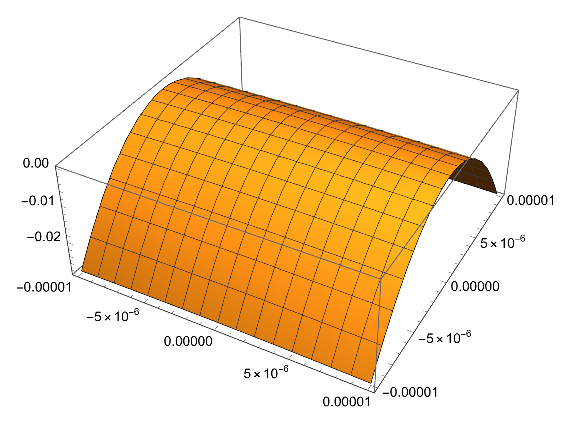
\includegraphics[width=.5\textwidth]{./pdf/residual_taylor_order_1}
    \caption{Error analysis for a Taylor series of order 1}
    \label{fig:residual_taylor_order_1}
\end{figure}

\begin{figure}[H]
    \centering
    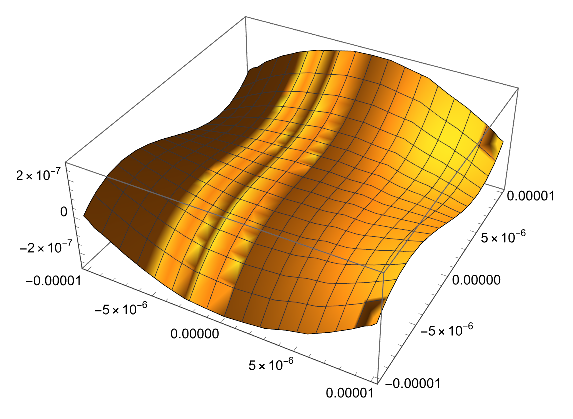
\includegraphics[width=.5\textwidth]{./pdf/residual_taylor_order_2}
    \caption{Error analysis for a Taylor series of order 2}
    \label{fig:residual_taylor_order_2}
\end{figure}

\begin{figure}[H]
    \centering
    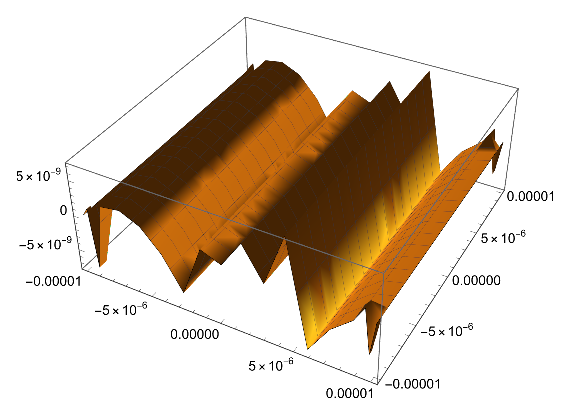
\includegraphics[width=.5\textwidth]{./pdf/residual_taylor_order_3}
    \caption{Error analysis for a Taylor series of order 3}
    \label{fig:residual_taylor_order_3}
\end{figure}

As we can see, around the point $\vec{u} = \vec{0}$, the error is negligible for both the approximations.
However, as we move away from the point $\vec{u} = \vec{0}$, the error introduced by the linearization increases.

In particular, we can see that the error introduced by the linearization decreases as we increase the order of the Taylor series expansion.

\section{Numerical solution}
\label{sec:numerical_solution}

We can now proceed to solve the system of equations ${\vec{P}} = f({\vec{u}})$ numerically.
To do so, we will use two different combined methods, in the form of Predictor-Corrector, that are:

\begin{itemize}
    \item Euler and Newton-Raphson
    \item Euler and modified Newton-Raphson
\end{itemize}

Just as a review of the methods, we report in the following the algorithms for the tree methods applied to a 2D problem (easily extendable to 3D).

Notice that with the symbol $[K_t]$ we are referring to the tangent stiffness matrix, that by definition is:

\begin{equation}
    [K_t] = \frac{\partial \vec{P_{ext}}}{\partial \vec{u}}
    =
    \begin{bmatrix}
        \frac{\partial P_{ext,x}}{\partial u} & \frac{\partial P_{ext,x}}{\partial v} \\
        \frac{\partial P_{ext,y}}{\partial u} & \frac{\partial P_{ext,y}}{\partial v}
    \end{bmatrix}
    \label{eq:tangent_stiffness_matrix}
\end{equation}

Instead, with the symbol $\vec{R}$ we are referring to the residual vector, that by definition is:

\begin{equation}
    \vec{R} = \vec{F_{int}} - \vec{P_{ext}}
    \label{eq:residual_vector}
\end{equation}

Since we will work in a discretized domain, we will use the subscript $n$ to refer to the current iteration, and the subscript $n+1$ to refer to the next iteration.
So $[K_{t,n}]$ and $\vec{R_n}$ will simply be the tangent stiffness matrix and the residual vector evaluated at the current iteration with the associated values of $\vec{u}$.

\subsection{Euler}

Used as predictor, the Euler method is defined as:

\begin{equation}
    {\vec{u}_{n+1}} = {\vec{u}_n} + [K_{t,n}]^{-1} * {\vec{P_{ext,n}}}
    \label{eq:euler_method}
\end{equation}


\subsection{Newton-Raphson}

Used as corrector, the Newton-Raphson method is defined as:

\begin{equation}
    {\vec{u}_{n+1}} = {\vec{u}_n} - [K_{t,n}]^{-1} * {\vec{R_n}}
    \label{eq:newton_raphson_method}
\end{equation}

\subsection{Modified Newton-Raphson}

Similarly to the Newton-Raphson method, the modified Newton-Raphson method is defined as:

\begin{equation}
    {\vec{u}_{n+1}} = {\vec{u}_n} - [K_{t,0}]^{-1} * {\vec{R_n}}
    \label{eq:modified_newton_raphson_method}
\end{equation}

Where $[K_{t,0}]$ is the tangent stiffness matrix evaluated at the first iteration.
\section{Implementation}
\label{sec:implementation}

For each of the previous models (\ref{eq:force_displacement_relationship},\ref{eq:taylor_series_expansion_order_1},\ref{eq:taylor_series_expansion_order_2},\ref{eq:taylor_series_expansion_order_3},\ref{eq:force_displacement_relationship_approximation_soft},\ref{eq:force_displacement_relationship_approximation_hard}) we can then compute the tangent stiffness matrix and the internal force vector as function of $\vec{u}$.
By applying the definition \ref{eq:tangent_stiffness_matrix} and \ref{eq:residual_vector} we are able to basically compute for each model two functions $f_{K_t}(\vec{u})$ and $f_{R}(\vec{u})$ that will return the tangent stiffness matrix and the residual vector evaluated at the current iteration referring to the displacement $\vec{u_n}$.

As an example, we report the functions $f_{K_t}(\vec{u})$ and $f_{R}(\vec{u})$ for the model \ref{eq:taylor_series_expansion_order_1}:

\begin{equation}
    f_{K_t}(\vec{u}) =
    \begin{bmatrix}
        \frac{\partial P_{ext,x}}{\partial u} & \frac{\partial P_{ext,x}}{\partial v} \\
        \frac{\partial P_{ext,y}}{\partial u} & \frac{\partial P_{ext,y}}{\partial v}
    \end{bmatrix}
    =
    \begin{bmatrix}
        \frac{\partial}{\partial u} \left( \frac{\text{A}_1 \text{E}_1}{L_1} \left( u - u_0 \right) \right) & \frac{\partial}{\partial v} \left( \frac{\text{A}_1 \text{E}_1}{L_1} \left( u - u_0 \right) \right) \\
        \frac{\partial}{\partial u} \left( \frac{\text{A}_2 \text{E}_2}{L_2} \left( v - v_0 \right) \right) & \frac{\partial}{\partial v} \left( \frac{\text{A}_2 \text{E}_2}{L_2} \left( v - v_0 \right) \right)
    \end{bmatrix}
    =
    \begin{bmatrix}
        \frac{\text{A}_1 \text{E}_1}{\text{L}_1} & 0                                        \\
        0                                        & \frac{\text{A}_2 \text{E}_2}{\text{L}_2}
    \end{bmatrix}
    \label{eq:tangent_stiffness_matrix_taylor_series_expansion_order_1}
\end{equation}

\begin{equation}
    f_{R}(\vec{u}) = \vec{F_{int}} - \vec{P_{ext}}
    \label{eq:residual_vector_taylor_series_expansion_order_1}
\end{equation}

\begin{equation}
    \vec{F_{int}} =
    \begin{bmatrix}
        \frac{\text{A}_1 \text{E}_1}{\text{L}_1} \left( u - u_0 \right) \\
        \frac{\text{A}_2 \text{E}_2}{\text{L}_2} \left( v - v_0 \right)
    \end{bmatrix}
    =
    \begin{bmatrix}
        \frac{\text{A}_1 \text{E}_1}{\text{L}_1} u \\
        \frac{\text{A}_2 \text{E}_2}{\text{L}_2} v
    \end{bmatrix}
    \label{eq:internal_force_vector_taylor_series_expansion_order_1}
\end{equation}

When it comes to \texttt{MATLAB} code, the functions $f_{K_{t,n}}(\vec{u_n})$ and $f_{F_{int,n}}(\vec{u_n})$ are implemented as follows:

\begin{lstlisting}[language=Matlab]
function [Kt, Fint] = model_taylor_1(U, geometry)

    [L1, A1, E1, L2, A2, E2] = decompose_geometry(geometry); % From a struct to variables
    [u, v] = decompose_u(U); % From a vector to variables

    Kt = [
        [A1.*E1.*L1.^(-1) 0];
        [0 A2.*E2.*L2.^(-1)]
        ];

    Fint = [
        A1.*E1.*L1.^(-1).*u;
        A2.*E2.*L2.^(-1).*v
        ];

end
\end{lstlisting}


\clearpage
\section{Results}

The numerical solution results for the problem described in \ref{sec:requests} are reported in the following table and figures.

\begin{figure}[H]
    \centering
    \csvautotabular{../Results/numerical_results.csv}
    \label{tab:results}
\end{figure}

\begin{figure}[H]
    \centering
    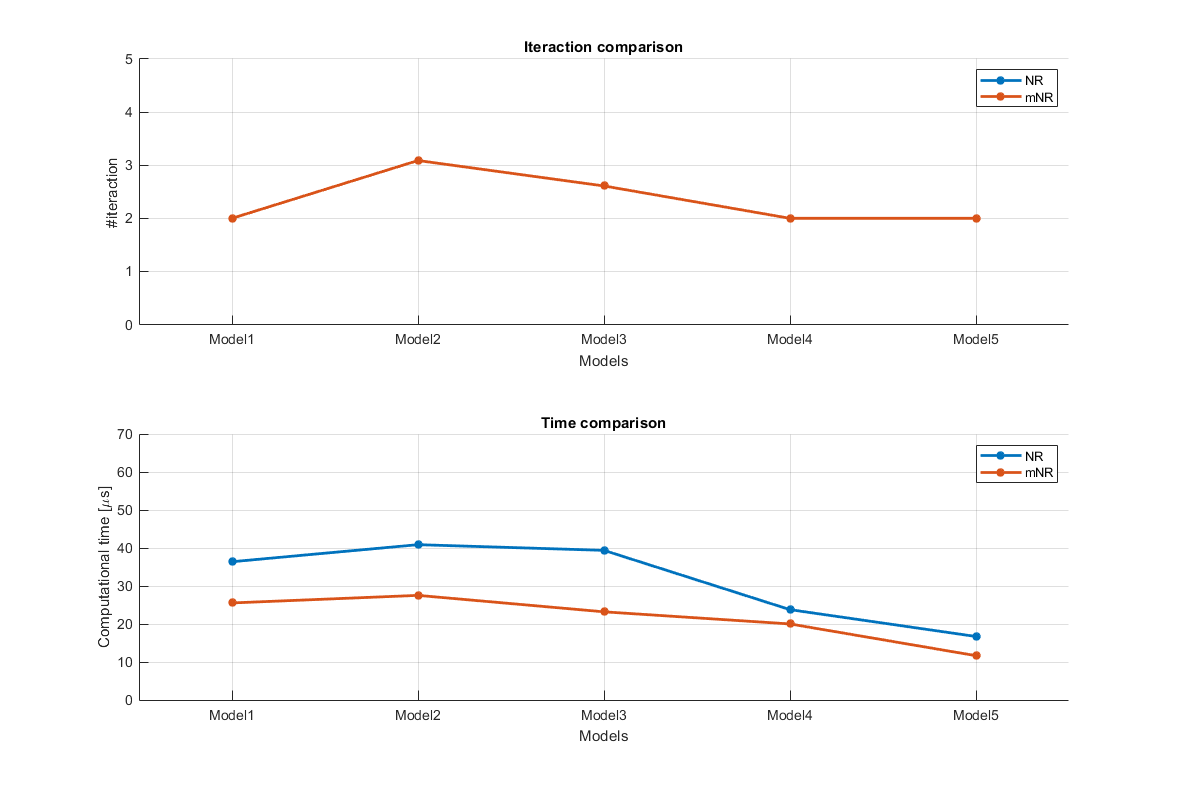
\includegraphics[width=.9\textwidth]{../Results/correctors_methods_comparison}
    \label{fig:correctors_methods_comparison}
\end{figure}

\begin{figure}[H]
    \centering
    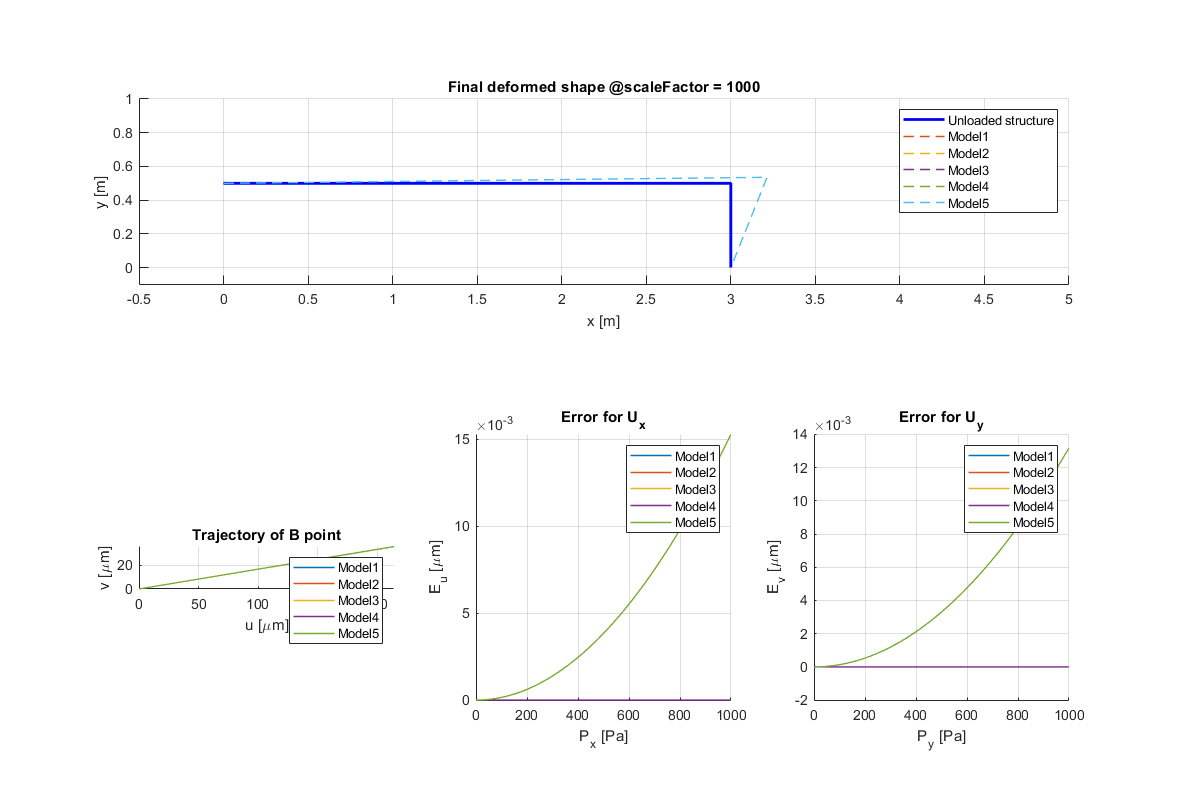
\includegraphics[width=.9\textwidth]{../Results/deformed_shape_analysis}
    \label{fig:deformed_shape_analysis}
\end{figure}

\clearpage
\appendix
\section{Mathematica code}
\label{sec:appendix}

Here follows the \texttt{Mathematica} notebook used for symbolic analysis of the equations.

\lstinputlisting[
    style=mathematica,
    language=Mathematica,
    caption=Mathematica notebook used for symbolic analysis of the equations.,
    firstline=1,
    lastline=56
]{files/notebook.txt}

\end{document}
